\section{Language Overview}
\label{sec:overview}

\begin{figure}
  \centering
  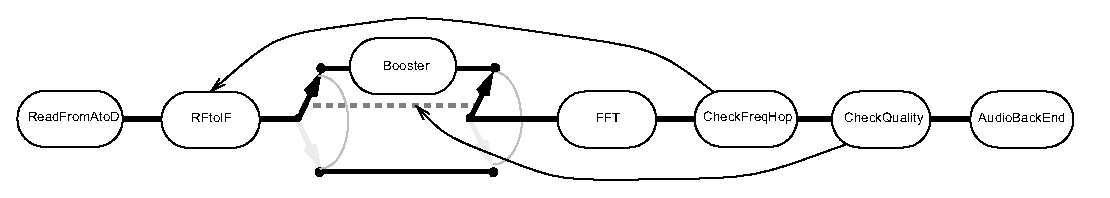
\includegraphics[width=\columnwidth]{Radio.eps}
  \caption{A block diagram of our frequency-hopping software radio.}
  \label{fig:radiodiagram}
%  \makeline
\end{figure}

StreamIt  includes  stream-specific  abstractions and  representations
that are designed to improve programmer productivity in the domain of
streaming   applications.   StreamIt   programs  are   represented  as
hierarchical  stream  graphs   consisting  of  \emph{filters}  as  the
fundamental processing  blocks. This section
presents the StreamIt 2.0 syntax for describing filters and the stream
graph.

\begin{figure}
  \centering
  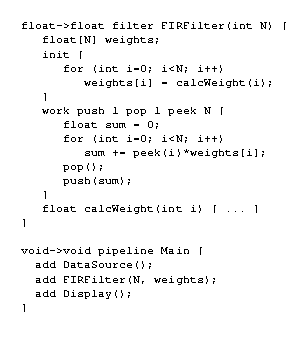
\includegraphics{fir-streamit.eps}
  \caption{An FIR filter in StreamIt.}
  \label{fig:firstreamit}
  \makeline
\end{figure}

\begin{figure}[t]
\vspace{-6pt}
~~
\begin{minipage}{0.46in}
\centering
\psfig{figure=pipeline.eps,width=0.46in} \\
\end{minipage} 
~
\begin{minipage}{1.3in}
\centering
\psfig{figure=splitjoin.eps,width=1.3in} \\
\end{minipage}
~
\begin{minipage}{1.02in}
\centering
\psfig{figure=feedback.eps,width=1.02in} \\
\end{minipage} 
\\ ~ \\ {\bf \protect\small (a) A pipeline. ~~~~(b) A splitjoin. ~~~~(c) A feedbackloop.}
\caption{Stream structures supported by StreamIt.}
\label{fig:structuresp}
\vspace{-14pt}
\vspace{-6pt}
\makeline
\end{figure}

% \begin{figure}
% \centering
% \subfigure[A pipeline.]{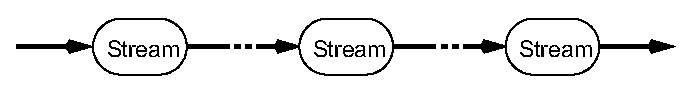
\includegraphics[width=1.8in]{basic-pipeline.eps}}
% \subfigure[A split-join.]{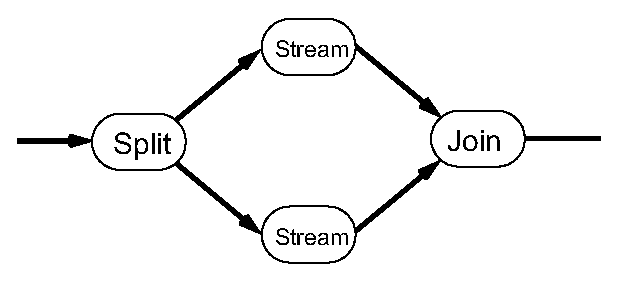
\includegraphics[width=1.8in]{basic-splitjoin.eps}}
% \subfigure[A feedback loop.]{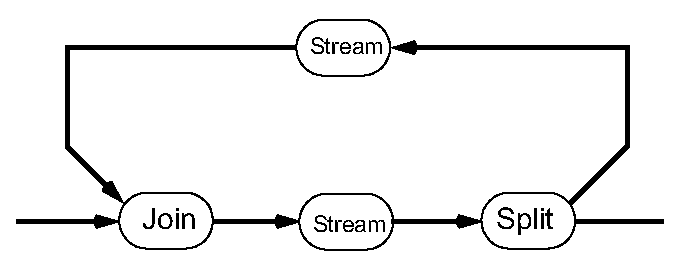
\includegraphics[width=1.8in]{basic-feedback.eps}}
% \caption{Stream structures supported by StreamIt.}
% \label{fig:structuresp}
% \end{figure}

\subsection{Filters}

The basic unit of computation  in StreamIt is the \texttt{filter}.  An
example   of  a   \texttt{filter}   from  our   software  radio   (see
Figure~\ref{fig:radiodiagram})  is  the  \texttt{FIRFilter}, shown  in
Figure~\ref{fig:firstreamit}.  Each  filter has an  input channel from
which it  reads data, and an  output channel to which  it writes data.
The filter also contains a \texttt{work} function, which describes the
filter's most fine grained execution step in the steady state.  Within
the \texttt{work} function, a  filter can communicate with neighboring
blocks over implicit channels that support three intuitive operations:
1) \texttt{pop()}  removes an  item from  the end  of the  channel and
returns its value, 2) \texttt{peek($i$)} returns the value of the item
$i$ spaces  from the end  of the channel  without removing it,  and 3)
\texttt{push($x$)}  writes  $x$ to  the  front  of  the channel.   The
argument $x$ is  passed by value; if it is an  object, a separate copy
is enqueued  on the  channel. Currently, the  number of  items peeked,
popped, and pushed by each filter must be constant from one invocation
of the \texttt{work}  function to the next.  In  fact, as described in
the sequel,  the input and  output rates are  declared as part  of the
\texttt{work} function declaration; a  violation of the declared rates
results in a runtime error  and the subsequent behavior of the program
is undefined. We plan to support variables input and output rates in a
future version of StreamIt.

Each filter also contains an  \texttt{init} function that is called at
the  time  of  initialization.   This  function  allows  the  user  to
establish the initial state of the filter.  For example, the FIRFilter
records  \texttt{weights}: the coefficients  used for  filtering.  The
\texttt{init} function  may not push,  pop, or peek items;  however, a
filter may also declare a \texttt{prework} function which is called in
place of the normal \texttt{work}  function on the first iteration.  A
filter   is  instantiated   using   \texttt{add},  \texttt{body},   or
\texttt{loop}  statements, and  the \texttt{init}  function  is called
implicitly  with   the  same  arguments   that  were  passed   in  the
instantiating statements.

Each filter has  a fixed input type, output type,  and I/O rates.  The
input  and  output   types  are  specified  as  part   of  the  filter
declaration;  the sample  \texttt{FIRFilter} has  an input  and output
type         of         \texttt{float},         represented         as
\texttt{float}~$\rightarrow$~\texttt{float}.   The I/O rates  are declared
as part of the work function.   Any expression that can be resolved to
a constant at compile time is a  valid I/O rate.  The peek rate may be
omitted if it is the same as the pop rate.

\begin{figure}
\centering
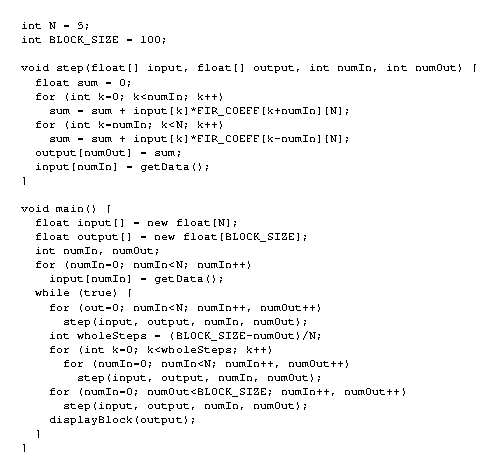
\includegraphics{fir-proc.eps}
\caption{An optimized FIR filter in a procedural language.  A
  complicated loop nest is required to avoid mod functions and to use
  memory efficiently, and the structure of the loops depends on the
  data rates (e.g., BLOCK\_SIZE) within the stream.  An actual
  implementation might inline the calls to \texttt{step}.}
\label{fig:firprocedural}
\end{figure}

\begin{figure}
\centering
\includegraphics{fir-object.eps}
\caption{An FIR filter in an object oriented language.  A ``pull
  model'' is used by each filter object to retrieve a chunk of data
  from its source, and straight-line code connects one filter to
  another.}
\label{fig:firobject}
\end{figure}

\label{sec:oo-rat}
\emph{Rationale.}  StreamIt's representation of a filter is an
improvement over general-purpose languages.  In a procedural language,
the analog of a filter is  a block of statements in a complicated loop
nest  (see   Figure~\ref{fig:firprocedural}).   This  representation  is
unnatural for expressing the feedback and parallelism that is inherent
in  streaming systems.  Also,  there is  no clear  abstraction barrier
between one  filter and another, and high-volume  stream processing is
muddled with global variables and control flow.  The loop nest must be
re-arranged if  the input  or output ratios  of a filter  change, and
scheduling optimizations further inhibit  the readability of the code.
In contrast, StreamIt  places the filter in its  own independent unit,
making explicit  the parallelism and  inter-filter communication while
hiding  the grungy  details of  scheduling and  optimization  from the
programmer.

Alternatively, one could use an object-oriented language to  implement a stream
abstraction (see  Figure~\ref{fig:firobject}).  This avoids  some of the
problems associated  with a procedural loop nest,  but the programming
model is again complicated by efficiency concerns.  That is, a runtime
library usually  executes filters according  to a pull model,  where a
filter operates  on a block of  data that it retrieves  from the input
channel.  The  block size is often  optimized for the cache  size of a
given architecture, thus hampering portability.  Moreover, operating on
large-grained blocks  obscures the fundamental  fine-grained algorithm
that is visible in a StreamIt  filter.  Thus, the absence of a runtime
model  in  favor  of   automated  scheduling  and  optimization  again
distinguishes StreamIt.

\subsection{Connecting Filters}
\label{sec:connecting}

\begin{figure}
\centering
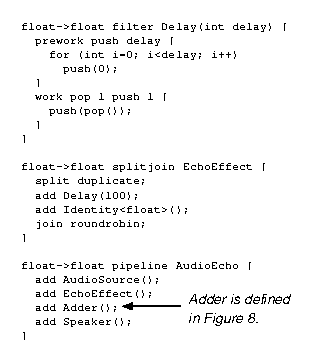
\includegraphics{echo.eps}
\caption{An echo effect in StreamIt.  Extra items are pushed on to
  \texttt{Delay}'s output tape in the \texttt{prework} function to
  cause the delay.}
\label{fig:echo}
\end{figure}

\begin{figure}
\centering
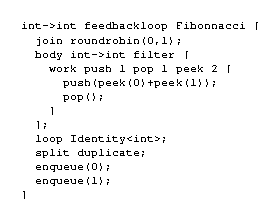
\includegraphics{fib-streamit.eps}
\caption{A \texttt{feedbackloop} version of Fibonnacci.}
\label{fig:feed}
\end{figure}

StreamIt provides three constructs for composing filters into a
communicating network. They are \texttt{pipeline}, \texttt{splitjoin}, and
\texttt{feedbackloop} (see Figure~\ref{fig:structuresp}).  Each
structure  specifies a pre-defined  way of  connecting filters  into a
single-input,  single-output   block,  henceforth  refereed   to  as  a
``stream''.  That is, a stream is any instance of a \texttt{filter},
\texttt{pipeline}, \texttt{splitjoin}, or \texttt{feedbackloop}. 
Generally,  a  pipeline is  for  building  a  sequence of  streams,  a
split-join is for running streams  in parallel, and a feedback loop is
or introducing cycles in the  stream graph.  Every StreamIt program is
a hierarchical composition of these stream structures.

The \texttt{pipeline} construct is for building a sequence of
streams.  The body of a pipeline is a sequence of statements that are
called upon its instantiation.  Component streams are added to the
pipeline via successive calls to \texttt{add}.  For example, in the
\texttt{AudioEcho} in Figure~\ref{fig:echo}, there are four streams in
the pipeline: an \texttt{AudioSource}, an \texttt{EchoEffect}, an
\texttt{Adder}, and a \texttt{Speaker}.  This sequence of statements
automatically connects the four streams in the order specified.
Thus, there is no \texttt{work} function in a pipeline, as the
component streams fully specify the behavior.  The channel types and
data rates are also implicit from the connections.

% Each of the stream constructs can either be executed on its own, or
% embedded in an enclosing stream structure.  The \texttt{AudioEcho} can
% execute independently, since the first component consumes no items and
% the last component produces no items.  However, the
% \texttt{EchoEffect} must be used as a component, since the first
% stream inputs items and the last stream outputs items.  When a stream
% is embedded in another construct, the first and last components of the
% stream are implicitly connected to the stream's neighbors in the
% parent construct.

% The input and output channels of the Pipeline itself are connected to
% the first and last component streams, respectively.  Thus, a Pipeline
% can be embedded in another stream construct, and the channels of the
% first and last components are implicitly connected to the Pipeline's
% neighbors in the parent construct.  Alternatively, if a Pipeline
% consumes no items from its input and produces no items to its output (as
% is the case with {\tt AudioEcho}), then the Pipeline can be run as an
% independent unit--a toplevel StreamIt program.  Any Pipeline, SplitJoin,
% or FeedbackLoop that has consumes no input and produces no output is a
% valid toplevel program in StreamIt.

% Of course, there are a number of semantic restrictions on the
% construction of Pipelines.  For each pair of streams that is
% connected, the output type of the first stream must match the input
% type of the next.  Also, there must be non-zero production and
% consumption rates along the inner connections of a Pipeline, such that
% data flows through the entire pipe.  We omit a full discussion of
% semantic checking in StreamIt due to lack of space.

The  \texttt{splitjoin}  construct  is  used  to  specify  independent
parallel streams that diverge  from a common \emph{splitter} and merge
into a  common \emph{joiner}.  As in  a pipeline, the  components of a
split-join are  specified with successive calls  to \texttt{add}.  For
example,  the \texttt{EchoEffect}  in  Figure~\ref{fig:echo} adds  two
streams that run in parallel, the first is a \texttt{Delay} filter and
the other is an identity filter.

The splitter specifies how items  from the input of the split-join are
distributed to the parallel components.  For simplicity, we allow only
compiler-defined splitters, of which there are two types:
\texttt{duplicate}, which replicates each data item and sends a copy
to each parallel stream, and \texttt{roundrobin($i_1$, $i_2$, $\dots$,
$i_k)$}, which sends the first $i_1$ data items to the stream that was
added first,  the next $i_2$ data  items to the stream  that was added
second,  and   so  on.   As   shorthand,  \texttt{roundrobin($i$)}  is
equivalent  to   \texttt{roundrobin($i$,  $i$,  $i$,   $\dots$)}.   An
unadorned \texttt{roundrobin} is equivalent to \texttt{roundrobin(1)},
and  \texttt{roundrobin(0)}  may  be  used  if none  of  the  parallel
components require any  input, and there are no  input items to split.
Note that \texttt{roundrobin} can function as an exclusive selector if
one or more of the weights are zero.

% \begin{enumerate}
% \item {\tt Duplicate}, which replicates each data item and sends a copy to each
% parallel stream.
% \item {\tt RoundRobin($i_1$, $i_2$, $\dots$, $i_k)$},
% which sends the first $i_1$ data items to parallel stream 1, the next
% $i_2$ data items to parallel stream 2, and so on.  If the weights are
% ommitted, then they are assumed to be equal to one for each stream.  Note
% that RoundRobin can function as an exclusive selector if one or more of the
% weights are zero.
% \item {\tt Null}, which means that none of the parallel components require
% any input, and there are no input items to split.
% \end{enumerate}

Similarly,  the joiner  is used  to indicate  how the  outputs  of the
parallel  streams  are  interleaved  on  the  output  channel  of  the
split-join.  The  only supported joiner  is \texttt{roundrobin}, which
is analogous to a round-robin splitter.

The   splitter  and  joiner   types  are   specified  with   calls  to
\texttt{split}      and     \texttt{join},      respectively.      The
\texttt{EchoEffect}  uses  a  duplicate  splitter so  that  each  item
appears directly---via the identity filter---and as an echo---via the
\texttt{Delay} filter. The round-robin joiner interleaves the
immediate signals  with the  delayed ones.  In  \texttt{AudioEcho}, an
\texttt{Adder} is used to combine each pair of interleaved signals.

The \texttt{feedbackloop} construct provides a way to create cycles in
the    stream    graph.      The    \texttt{Fibonacci}    stream    in
Figure~\ref{fig:feed}  illustrates the  use of  this  construct.  Each
feedback loop  contains: 1) a body  stream, which is  the block around
which  a backward  ``feedback  path''  is being  created,  2) a  loop
stream, which can perform some computation along the feedback path, 3)
a splitter, which  distributes data between the feedback  path and the
output  channel at  the bottom  of the  loop, and  4) a  joiner, which
merges items  between the feedback path  and the input  channel at the
top  of  the  loop.   These  components are  specified  via  calls  to
\texttt{body},   \texttt{loop},  \texttt{split},   and  \texttt{join},
respectively.
%
% Each FeedbackLoop contains: 1) a
% joiner, which is at the top of the loop and merges the outside input
% stream with the ``feedback path'' from downstream, 2) a body stream,
% which comprises the forward path of the loop, 3) a splitter, which
% distributes data between the output channel and the feedback path, and
% 4) a loop stream, which can perform some computation along the feedback
% path.  These components are specified from within the {\tt init}
% function via calls to {\tt setJoiner}, {\tt setBody}, {\tt setSplitter},
% and {\tt setLoop}, respectively.  
%
The splitters and joiners can  be any of those for \texttt{splitjoin},
with   the   exception  of   \texttt{roundrobin(0)}.    The  call   to
\texttt{loop} may be omitted if no computation is performed along the
feedback path.

The  feedback loop  has special  semantics  when the  stream is  first
executed.   The loop's  joiner  needs inputs  from  its feedback  path
before  it can fire.   These inputs  are provided  by \texttt{enqueue}
statements within the body of the loop.

Evident in the \texttt{Fibonnacci} example of Figure~\ref{fig:feed} is
another  feature   of  the  StreamIt   syntax:  \emph{inlining}.   The
definition  of  any  stream  can  be  inlined  at  the  point  of  its
instantiation, thereby preventing the  definition of many small stream
structures that are used only  once, and, moreover, providing a syntax
that  reveals  the hierarchical  structure  of  the  streams from  the
indentation level of the code.

\emph{Rationale.}  StreamIt differs from other languages in that it
imposes a well-defined structure on the streams; all stream graphs are
built out of a hierarchical composition of pipelines, split-joins, and
feedback  loops.   This is  in  contrast  to  other environments  that
generally regard a  stream as a flat and  arbitrary network of filters
that are  connected by channels.   Arbitrary graphs are very  hard for
the compiler  to analyze,  and equally difficult  for a  programmer to
describe.  Most  programmers either resort to  straight-line code that
links one filter  to another (thereby obscuring the  stream graph), or
they use  an ad-hoc graphical  programming environment that  admits no
good textual representation.

In contrast, StreamIt affords a clean textual representation of stream
graphs,  and the  comparison  of StreamIt's  structure with  arbitrary
stream  graphs may  be likened  to the  difference  between structured
control  flow  and  GOTO   statements:  although  the  structure  may
occasionally restrict the expressiveness  of the programmer, the gains
in  robustness,  readability,   and  compiler  analysis  are  immense.
Furthermore, the  graphical programming environment  we have developed
for StreamIt has the advantage  that every stream graph corresponds to
a precise textual  counterpart that is easily edited  by a programmer.
Further,  the hierarchical  structure of  the stream  graph simplifies
visualization,  and  hence  the  graphical development  environment  is
better suited for large scale application development.

%On first glance, the statements within StreamIt {\tt init} function
%might appear more like a verbose API than a novel language.  However,
%it was actually a careful design decision to specify all ``stream
%configuration information'' via function calls from within the {\tt
%init} functions.  While the current syntax is somewhat tedious, there
%is great flexibility in this approach, since the user can intermix
%configuration directives with statements that calculate the
%configuration parameters.  This allows for fully parameterized graph
%construction--the FFT stream in Figure \ref{fig:radiocode} inputs a
%parameter {\tt N} and adjusts the number of butterfly stages
%appropriately.  This further improves the modularity and readability
%of the code.

\subsection{Messages}

% \begin{figure}
% \vspace{-12pt}
% \begin{minipage}{61mm}
% \psfig{figure=code.eps,width=60mm}
% \end{minipage}
% \begin{minipage}{61mm}
% \psfig{figure=code2.eps,width=63.92mm}
% \end{minipage}
% \vspace{-12pt}
% \caption{A StreamIt implementation of the Trunked Radio receiver.  Arrows denote the paths of messages.}
% \end{figure}

% \begin{figure}[h]
% \vspace{-12pt}
% \psfig{figure=messaging-code.eps,width=675.44pt}
% \vspace{-18pt}
% \caption{The frequency-hopping of our software radio illustrates StreamIt's messaging system.  In {\tt TrunkedRadio}, a {\tt Portal} is created to hold the message target, {\tt rf2if}.  Then, {\tt CheckFreqHop} uses the {\tt Portal} to send a frequency-change message.
% \protect\label{fig:portal-code}}
% \vspace{-18pt}
% \end{figure}

StreamIt provides a dynamic messaging system for passing irregular,
low-volume control information between filters and streams.  Messages
are sent from within the body of a filter's \texttt{work} function,
perhaps to change a parameter in another filter.  For example, in our
software radio example, the
\texttt{CheckFreqHop} stage sends a message upstream to change the
frequency of the receiver if it detects that the transmitter is about
to change frequencies.  The sender can continue to execute while the
message is en route, and the target method will be invoked
in the receiver with the specified arguments when the message
arrives.  Since message delivery is asynchronous, there can be no
return value; only void methods can be message targets.

%\paragraph{Message timing.} 
The central aspect of the messaging system is a
sophisticated timing  mechanism that allows filters to  specify when a
message is  received relative to  the flow of information  between the
sender   and  the   receiver.   Recall   that  each   filter  executes
independently,  without any  notion of  global time.   Thus,  the only
meaningful notion of time for any two filters is in terms of the data
items that are passed through the streams from one to the other.

In StreamIt, one can specify a range of latencies for each message
delivery.  This latency is measured in terms of an information
``wavefront'' from one filter to another.  For example, in the
\texttt{CheckFreqHop} example of Figure~\ref{fig:radiodiagram}, the
sender indicates an interval of  latencies between $4N$ and $6N$.  Due
to  space limitations,  we cannot  define this  notion  precisely (see
\cite{streamittech620,streamittech622} for  the formal semantics), but
the general idea  is simple: the receiver is invoked  when it sees the
information wavefront that  the sender sees in $4N$  to $6N$ execution
steps.

% In some cases, the ability to synchronize the arrival of a message
% with some element of the data stream is very important.  For example,
% \texttt{CheckFreqHop} knows that the transmitter will change the
% frequency between $4N$ and $6N$ steps later, in terms of the frame
% that \texttt{CheckFreqHop} is inputting.  To ensure that the radio
% changes frequencies at the same time--so as not to lose any data at
% the old or new frequency--\texttt{CheckFreqHop} instructs the receiver to
% switch frequencies when the \emph{receiver} sees one of the last data
% items at the old frequency.

% If the receiver of a message is a stream instead of a filter, then the
% message delivery is timed with respect to the first (most upstream)
% filter in the stream.  We are still formalizing the message delivery
% semantics in cases where the receiver is a stream that has no unique
% first filter (e.g., a SplitJoin with NULL splitter).  Note that the
% stream itself can receive a message even though the timing is in terms
% of filter-to-filter communication.
%
%\paragraph{Portals for broadcast messaging.}  

StreamIt also supports
modular broadcast messaging.  When a sender wants to send a message
that will invoke method $M$ of the receiver $R$ upon arrival, it does
not call $M$ on the object $R$.  Rather, it calls $M$ on a
\emph{portal} of which $R$ is a member.  Portals are typed containers
that forward all messages they receive to the elements of the
container.  Portals could be useful in cases when a component of a
filter library needs to announce a message (e.g., that it is shutting
down) but does not know the list of recipients; the user of the
library can pass to the filter a portal containing all interested
receivers.  As for message delivery constraints, the user specifies a
single time interval for each message, and that interval is
interpreted separately (as described above) for each receiver in the
portal.

\emph{Rationale.}  Stream programs present a challenge in that filters
need  regular, high-volume data transfer as well as irregular, low-volume
control communication.  Moreover, there is the problem of reasoning
about the relative ``time'' between filters when they are running
asynchronously and in parallel.

A different approach to messaging  is to embed control messages in the
data  stream instead  of providing  a separate  mechanism  for dynamic
message passing.  This does have the effect of associating the message
time with a  data item, but it is  complicated, error-prone, and leads
to unreadable code.  Further, it  could hurt performance in the steady
state  (if each filter  has to  check whether  or not  a data  item is
actual  data or  control, instead)  and may  also  complicate compiler
analysis.  Finally, one can't  send messages upstream without creating
a separate data channel for them to travel in.

Another solution is to treat messages as synchronous method calls.
However, this delays the progress of the stream when the message is en
route, thereby degrading the performance of the program and
restricting the compiler's freedom to reorder filter executions.  

We feel that the StreamIt messaging model is an advance in that it
separates the notions of low-volume and high-volume data transfer---both
for the programmer and the compiler---without losing a well-defined
semantics where messages are \emph{timed} relative to the high-volume
data flow.  Further, by separating message communication into its own
category, fewer connections are needed for steady-state data transfer
and the resulting stream graphs are more amenable to structured stream
programming.

\subsection{Re-Initialization}
\label{sec:reinit}

One of the characteristics of a streaming application is the need to
occasionally modify the structure of  the stream graph.
StreamIt allows these changes through a re-initialization mechanism
that is integrated with its messaging model.  If a sender targets a
message at the \texttt{init} function of a stream or filter $S$, then
when the message arrives, it re-executes the initialization code and
replaces $S$ with a new version of itself.  However, the new version
might have a different structure than the original if the arguments to
the \texttt{init} call on re-initialization were different than during
the original initialization.

When an \texttt{init} message arrives, it does not kill all of the
data that is in the stream being re-initialized.  Rather, it
\emph{drains} the stream until the wavefront of information (as
defined for the messaging model) from the top of the stream has
reached the bottom.  The draining occurs without consuming any data
from the input channels to the re-initialized region.  Instead, a
\texttt{drain} function of each filter is invoked to provide input
when its other input source is frozen.  (Each filter can override the
\texttt{drain} function as part of its definition.)  If the programmer
prefers to kill the data in a stream segment instead of draining it,
this can be indicated by sending an extra argument to the message
portal with the re-initialization message.

\emph{Rationale.}  Re-initialization is a headache for stream
programmers because---if done manually---the entire runtime system could
be put on hold to re-initialize a portion of the stream.  The
interface to starting and stopping streams could be complicated when
there is not an explicit notion of initialization time vs.
steady-state execution time, and ad-hoc draining techniques could risk
losing data or deadlocking the system.

StreamIt improves on this situation by abstracting the
re-initialization process from the user.  That is, no axillary
control program is needed to drain the old streams and create the new
structure; the user need only trigger the reinitialization process
through a message.  Additionally, any hierarchical stream construct
automatically becomes a possible candidate for re-initialization, due
to the well-defined stream structure and the simple interface with the
\texttt{init} function.  Finally, it is easy for the compiler to
recognize stream re-initialization possibilities and to account for
all possible configurations of the stream flow graph during analysis
and optimization.

%\subsection{Latency Constraints}

%Lastly, StreamIt provides a simple way of restricting the latency of
%an information wavefront in traveling from the input of one filter to
%the output of a downstream filter.  Issuing the directive
%\texttt{MAX\_LATENCY(A, B, n)} from within \texttt{init} means that
%$A$ can only execute up to the wavefront of information that $B$ will
%see after $n$ invocations of its own work function.
